\documentclass[a4paper,12pt]{scrreprt}
    %% Used for changing geometry of the page
    %% Cover page text cannot overlay cover sketching/style 
    %% https://ctan.org/pkg/geometry?lang=en
\usepackage{geometry}
    %% Changes language of some packages protocols
    %% e.g., when captioning images: Figure 1. -> Figura 1.
    %% https://ctan.org/pkg/babel?lang=en
\usepackage[portuguese]{babel}
    %% Used for special fonts
    %% Cannot be compiled with pdflatex
    %% https://ctan.org/pkg/fontspec?lang=en
\usepackage{fontspec}
    %% Arial FONT
    %%\setmainfont{Arial}
    \setmainfont{Liberation Sans}

    %% More colors and color options
    %% https://ctan.org/pkg/xcolor?lang=en
    %% https://ctan.org/pkg/colortbl?lang=en
\usepackage{xcolor,colortbl}
    %% More tabular options, like dashed/dotted lines
    %% https://ctan.org/pkg/arydshln?lang=en
\usepackage{arydshln}
    %% List of acronyms
    %% https://ctan.org/pkg/nomencl?lang=en
\usepackage[intoc]{nomencl}
    %% Must be called to init nomencl environment  
    \makenomenclature
    %% More images options/settings
    %% https://ctan.org/pkg/graphicx?lang=en
\usepackage{graphics}
    %% Defining subdirectories to image path enviornment
    %% \graphicspath{{sub1}{sub2}...{subN}}
    \graphicspath{{images}}
    
    %% used to handle cross-referencing commands in LaTeX to produce hypertext links in the document
    %% https://ctan.org/pkg/hyperref?lang=en
\usepackage{hyperref}
    %% math environments
    %% https://ctan.org/pkg/amsmath?lang=en

    %% settings
    \hypersetup{
        colorlinks,
        citecolor=black,
        filecolor=black,
        linkcolor=black,
        urlcolor=black
    }

\usepackage{amsmath}
    %% Defining backgrouns, used to make the cover
    %% https://ctan.org/pkg/background?lang=en
\usepackage[some]{background}
    %% Used to make drawings or complex graphics
    %% http://pgf.sourceforge.net/pgf_CVS.pdf
\usepackage{tikz}
% we want ER + above/below + left/right
\usetikzlibrary{calc}
\usepackage{float}

%% Defining sfdefault font and default font for document
\usepackage[indexing, style=authoryear]{biblatex}
\addbibresource{citations.bib}
\renewcommand{\familydefault}{\sfdefault}


%==========================================================================
% DOCUMENT
%==========================================================================

\begin{document}

\pagenumbering{gobble}

% builds the cover
%% Blue cover color
\definecolor{titlepagecolor}{RGB}{49,132,155}

%==========================================================================
% COLORED BAR ON THE LEFT SIDE
%==========================================================================

\backgroundsetup{
    scale=1, 
    angle=0, 
    opacity=1,
    contents={
        \begin{tikzpicture}[remember picture,overlay]
            \path [fill=titlepagecolor] 
                (current page.north west) -- ($(current page.north west) + (5,0)$)
                -- ($(current page.south west) + (5,0)$)-- (current page.south west); 
            \node[color=white] at ($(current page.south west) + (2.5,4)$) {\bfseries {\fontsize{120}{60} \textsf{ B}}};
            \node[color=titlepagecolor] at ($(current page.south west) + (5.8,4)$) {\bfseries {\fontsize{120}{60} \textsf{ D}}};
        \end{tikzpicture}
    }
}

%==========================================================================
% TITLE PAGE INFO
%==========================================================================

%% Changes values in this field to show information in the cover and back cover about your team/project


%% TITLE
\title{Mademoiselle Borges: Um Sistema de Bases de Dados para a Gestão de Eventos em Eventopolis}

%% AUTHORS
\author{
    Bruno Gi\~ao (A96544) %%% Bruno Dias da Gião
  \qquad
    Jo\~ao Pereira (A95375) %%% João Luís da Cruz Pereira
  \qquad
    Helena Salazar (A75635) %%% Maria Helena Alves Machado Marques Salazar
  \qquad
    Tiago Teixeira (A97666) %%% Tiago Emanuel Lemos Teixeira
}
%% Date

\date{Novembro, 2023}

%% Course
\newcommand{\Course}{Licenciatura em Ciências da Computação}

%% Department
%%% \newcommand{\Department}{Escola de Engenharia}

%% UniName
\newcommand{\UniName}{Universidade do Minho}

%% UniPic
\newcommand{\UniPic}{
\includegraphics[scale=0.09]{images/uminho.png}}

%% University 
\newcommand{\University}{
    \begin{flushleft}
        \UniPic
    \end{flushleft}
    \textcolor{gray}{\small\textbf{\textsf{\UniName}}}\par
    %%% \textcolor{gray!80!white}{\small{\textsf{\Department}}}\par
    \textcolor{gray!70!white}{\small{\textsf{\Course}}}
}

%% UC
\newcommand{\UC}{
    \begin{flushleft}
        \par\textcolor{titlepagecolor}{  \LARGE\textbf{\textsf{Unidade Curricular de \\ Bases de Dados}}}
    \end{flushleft}
}

%% School Year
\newcommand{\SchoolYear}{
    \small{\textsf{Ano Letivo de 2023/2024}}}


%% Define new command to show title, author and date
\makeatletter
\let\Title\@title
\let\Author\@author
\let\Date\@date
\makeatother

%==========================================================================
% CLASSIFICATION SECTION 
%==========================================================================

%% School Year
\newcommand{\ReceptionDate}{}
%% Responsible
\newcommand{\Responsible}{}
%% Evaluation
\newcommand{\Evaluation}{}
%% Observations
\newcommand{\Observations}{}





%% MAKETEMPLATE
\newcommand{\makecover}{

%==========================================================================
% BEGIN COVER PAGE 
%==========================================================================

%% Removes page number on footer
\thispagestyle{empty}

%% No indentation 
\setlength{\parindent}{0em}

%% Put Background defined on \backgroundsetup, in this page
\BgThispage

%% Changing geometry to prevent overlay with text
%% At the end of back cover, geometry is default with \restoregeometry
\newgeometry{top=5cm,left=6cm,right=3cm,bottom=2cm}

%% builds university info defined previously
\University
\vspace{1cm}
%% builds curricular unity info defined previously
\UC
%% builds school year info defined previously
\SchoolYear

\vspace*{4cm}
%% bigger space (i think its the default one) between paragraphs 
\setlength{\parskip}{1em}

%% builds title info defined previously
\par\textbf{\textsf{\huge\Title}}
\vspace{1cm}
%% builds author(s) info defined previously
\par\Author

\vspace{0.5cm}

%% builds date info defined previously
\par\Date
\restoregeometry
\pagebreak

%==========================================================================
% END COVER PAGE 
%==========================================================================

%==========================================================================
% BEGIN BACK COVER PAGE 
%==========================================================================

%% Removes page number on footer
\thispagestyle{empty}

% Changing look of lines in tabular environment 
% Dashed -> dotted 
%% length of dashes
\setlength\dashlinedash{0.3pt}
%% space between dashes
\setlength\dashlinegap{1.5pt}
%% width of dashes
\setlength\arrayrulewidth{1.1pt}


%% This values can be changed in the preamble
\begin{flushright}
\begin{tabular}{ :p{4cm}:p{4cm}: } 
\hdashline
Data de Recepção & \ReceptionDate \\ [2ex]
\hdashline
Responsável & \Responsible \\ [2ex]
\hdashline
Avaliação & \Evaluation \\ [2ex]
\hdashline
Observações & \Observations \\ [7ex]
\hdashline
\end{tabular}
\end{flushright}


\vspace{9cm}
\begin{flushleft}

%% builds title info defined previously
\par\textbf{\textsf{\huge\Title}}
\vspace{1cm}
%% builds author info defined previously
\par\Author

\vspace{0.5cm}

%% builds date info defined previously
\par\Date
\end{flushleft}

\pagebreak
%==========================================================================
% END BACK COVER PAGE 
%==========================================================================
}

\makecover

%% smaller footer and header size
\newgeometry{top=3cm,left=3cm,right=3cm,bottom=4cm}

%==========================================================================
% BEGIN OPCIONAL DEDICATÓRIA
%==========================================================================

%%\clearpage
%%\begin{center}
 %%   \thispagestyle{empty}
  %%  \vspace*{\fill}
    
  %%  $<<$/opcional Dedicatória$>>$
    
 %%   \vspace*{\fill}
%%\end{center}
%%\clearpage

%==========================================================================
% END OPCIONAL DEDICATÓRIA
%==========================================================================


%==========================================================================
% BEGIN ABSTRACT PAGE
%==========================================================================



%% Abstract name: \Large font size, flushed left and paragraph skip before abstract content
\renewenvironment{abstract}
 {\par\noindent\textbf{\Large\abstractname}\par\bigskip}
 {}

\begin{flushleft}
\begin{abstract}
    Neste trabalho, foi inicializado o processo do desenho de um Sistema de
    Bases de Dados na forma da contextualiza\c{c}\~ao do problema, visando
    criar uma \textit{blueprint} s\'olida e demonstrar que, efetivamente,
    \'e justificada a cria\c{c}\~ao do presente Sistema de Bases de Dados,
    o levantamento de requisitos de manipulação, descrição, e controlo e a
    conceptualização do problema com recurso a um diagrama conceptual
    (\textit{Entity-Relationship Diagram}).
    \par \textbf{\'Area de Aplicação}: Desenho e arquitectura de Sistemas de
    Bases de Dados.
    \par \textbf{Palavras-Chave}: Bases de Dados Relacionais,
    Defini\c{c}\~ao de Sistema, SQL, Diagrama Conceptual,
    Recolha de Requisitos.
\end{abstract}
\end{flushleft}


\pagebreak

%==========================================================================
% END ABSTRACT PAGE 
%==========================================================================

%==========================================================================
% BEGIN INDEXES PAGES
%==========================================================================

%% Changes table of content name
%% Portuguese babel default : "Conteúdo"
%% Personally I prefer "índice"
\renewcommand{\contentsname}{Índice}

\tableofcontents

\pagebreak

\listoffigures

\pagebreak

\listoftables

\pagebreak

%==========================================================================
% END INDEXES PAGES 
%==========================================================================


%==========================================================================
% BEGIN INTRODUCTION
%==========================================================================

%% Starting page numbering here
\pagenumbering{arabic}

\chapter{Introdução e Definição do Sistema}
     \section{Contextualização}

     Em Eventopolis, uma localidade remota no centro de uma densa floresta,
     a gestão dos eventos foi sempre baseada em \textit{outsourcing} ou métodos manuais,
     devido à escassez de recursos humanos e à existência de um monopólio na área de Bases
     de Dados (BD). Este monopólio era controlado por uma seita de ocultistas tecnológicos,
     os quais praticavam preços exorbitantes e limitavam o acesso a uma parte significativa
     das informações nas suas BD. Após uma revolta interna motivada pela insatisfação com a
     direção da empresa, alguns ex-membros, descontentes com a situação, optaram por adotar
     uma abordagem mais humanista e criar uma \textit{start-up} de Engenharia de Software em Eventopolis.
    
     Ao tomar conhecimento desta informação, o Professor Doutor Henrique Borges, responsável atual
     pela Gestão de Eventos na Câmara Municipal da cidade, prontamente identificou a
     oportunidade de mitigar os prejuízos significativos dos últimos anos ao estabelecer
     um contrato com a referida \textit{start-up} para a implementação de um Sistema de Bases de Dados (SBD) \textit{open-source}.
    
     O SBD seria batizado de ``Mademoiselle Borges'' em homenagem
     a Antoinette Borges, a antiga gestora de Eventos da Câmara Municipal de Eventopolis
     e esposa de Henrique Borges, que faleceu há alguns anos. Antoinette enfrentou uma pressão
     considerável ao depender da seita ou ao ser forçada a gerir manualmente os eventos com uma
     equipa de funcionários bastante limitada, desafios que foram fatores cruciais para o seu falecimento precoce.
   
     Para Henrique Borges, este projeto tem então um significado profundamente pessoal.
     Além de simplificar o funcionamento dos eventos, diminuindo a mortalidade deste posto de trabalho,
     a criação deste Sistema também reflete a sua vontade de fomentar a promoção da arte e da cultura
     na sua pequena cidade, algo que era o maior sonho da sua falecida esposa.
     Antoinette queria ver a transformação da modesta e isolada cidade numa capital cultural,
     uma aspiração que, infelizmente, apenas se concretizaria após o seu falecimento.
    
     Após a introdução do SBD, todos os eventos aprovados pela Câmara transformarão
     a cidade num cenário requintado que realça a estética do estilo \textit{Art Nouveau},
     o estilo artístico predileto da Mademoiselle, este estilo tira inspiração da vegetação exuberante,
     densa e colorida, característica das imensas florestas que rodeiam Eventopolis.
     O principal local de eventos será uma gigantesca estufa situada no parque central,
     construída no início do século anterior. Esta estrutura exibe uma cúpula central, vitrais coloridos
     e um esqueleto de ferro com linhas detalhadas e artísticas, que ao longo do tempo oxidaram,
     apresentando agora uma tonalidade verde clássica.

    \section{Fundamenta\c{c}\~ao}
    Considerando o modo prévio de gerir eventos em Eventopolis,
    onde o uso de serviços externos era considerado excessivamente dispendioso,
    e diante da escassez de recursos humanos para uma gestão manual, a única alternativa
    viável, na perspetiva de Henrique Borges, seria desenvolver um SBD interno.
    \section{Apresentação do Caso de Estudo}
    Este trabalho consistirá então na elaboração de um SBD que consiga, aptamente, ajudar Henrique Borges
    e a c\^amara municipal de Eventopolis a gerir e publicitar os seus eventos.
    
    \section{Motivação e Objectivos}
    O Professor Doutor Henrique Borges acredita que a introdu\c{c}\~{a}o de uma base de dados
    trar\'{a} sucesso aos eventos.

    Os objetivos mencionados abaixo s\~{a}o fundamentais para refletir este sucesso:
    \begin{itemize}
    \item Aumentar a capacidade de armazenamento de informa\c{c}\~{o}es;
    \item Saber em tempo real qual a previsão de afluência de cada evento, sendo assim possível
planear os eventos com maior precisão;
    \item Perceber quais são os colaboradores com melhor desempenho nas vendas, permitindo o
uso de incentivos para estimulá-los a alcançar novos patamares de vendas;
    \item Possibilitar uma gestão financeira mais abrangente e precisa;
    \item Garantir que é minimizada a possibilidade da capacidade do evento ser excedida;
    \item Obter, em tempo real, um registo preciso das compras de cada participante, bem como
identificar os itens mais vendidos tanto em eventos específicos quanto globalmente;
    \item Melhorar a organiza\c{c}\~{a}o de hor\'{a}rios para cada evento;
    \item Promover a cidade em \^{a}mbito nacional e internacional;
    \item Estimular a economia local por meio de inje\c{c}\~{a}o de capital na regi\~{a}o.
    \end{itemize}

        \section{Viabilidade}
        O Professor Doutor Henrique Borges defende que ao implementar um sistema de controlo de eventos
        será possível: 
        \begin{itemize}
          \item Recuperar, no final no primeiro semestre, $40\%$ das perdas anteriores e cerca de $20\%$
            do investimento inicial;
          \item Aumentar a participação nos eventos em $30\%$ no primeiro ano.
        \end{itemize}

        \section{Recursos}
             \subsubsection{Recursos Humanos}
             \begin{itemize}
               \item Pessoal de limpeza;
               \item Equipa de seguran\c{c}a;
               \item Vendedores;
               \item Equipa de multim\'edia;
               \item Funcion\'{a}rios da empresa de desenvolvimento;
               \item Potenciais Volunt\'arios.
             \end{itemize}
             \subsubsection{Recursos Materiais}
             \begin{itemize}
             \item{Hardware:}
               \begin{itemize}
                 \item 1 servidor fornecido pela \textit{start-up} com 128GiB;
                 \item 15 terminais ``burros'';
                 \item 10 computadores pessoais.
               \end{itemize}
             \item{Software:}
               \begin{itemize}
                 \item SGBD;
                 \item Aplicação de vendas e aprovisionamento;
                 \item Redes sociais para divulgar o calendários de eventos.
               \end{itemize}
             \end{itemize}
             \subsubsection{Equipa de Trabalho}
             \begin{itemize}
                 \item{\textbf{Pessoal Interno}}
                   Na equipa de gest\~ao de eventos da C\^amara Municipal de Eventopolis temos:
                   \begin{itemize}
                     \item{Professor Doutor Henrique Borges:} O coordenador principal da equipa;
                     \item{Maria Ivanovna Ivanova:} Colaboradora com experi\^encia em \textit{marketing} e co-coordenadora
                       da equipa;
                     \item{Herr Otto Mustermann:} Trabalhador \textit{part-time}.
                   \end{itemize}
                 \item{\textbf{Pessoal Externo}}
                   Já o pessoal externo, consiste na equipa de desenvolvimento da ``start-up'',
                   que seria constituída por 4 engenheiros, nomeadamente:
                   \begin{itemize}
                     \item Luke Bytespell;
                     \item Aurelius Cibern\'etico;
                     \item Bella Firewall;
                     \item Aurora Matrix.
                   \end{itemize}
             \end{itemize}
        \section{Plano de Execu\c{c}\~ao}
             Com o intuito de desenvolver atempadamente o SBD ``Mademoiselle Borges'', Henrique Borges e a equipa de desenvolvimento
              reuniram-se e elaboraram o seguinte esquema GANTT\footnote{(ver \ref{GANTT} e \ref{GANTT_c2} para esquema completo)}:
        \newpage
        \begin{figure}[h]
            \centering
            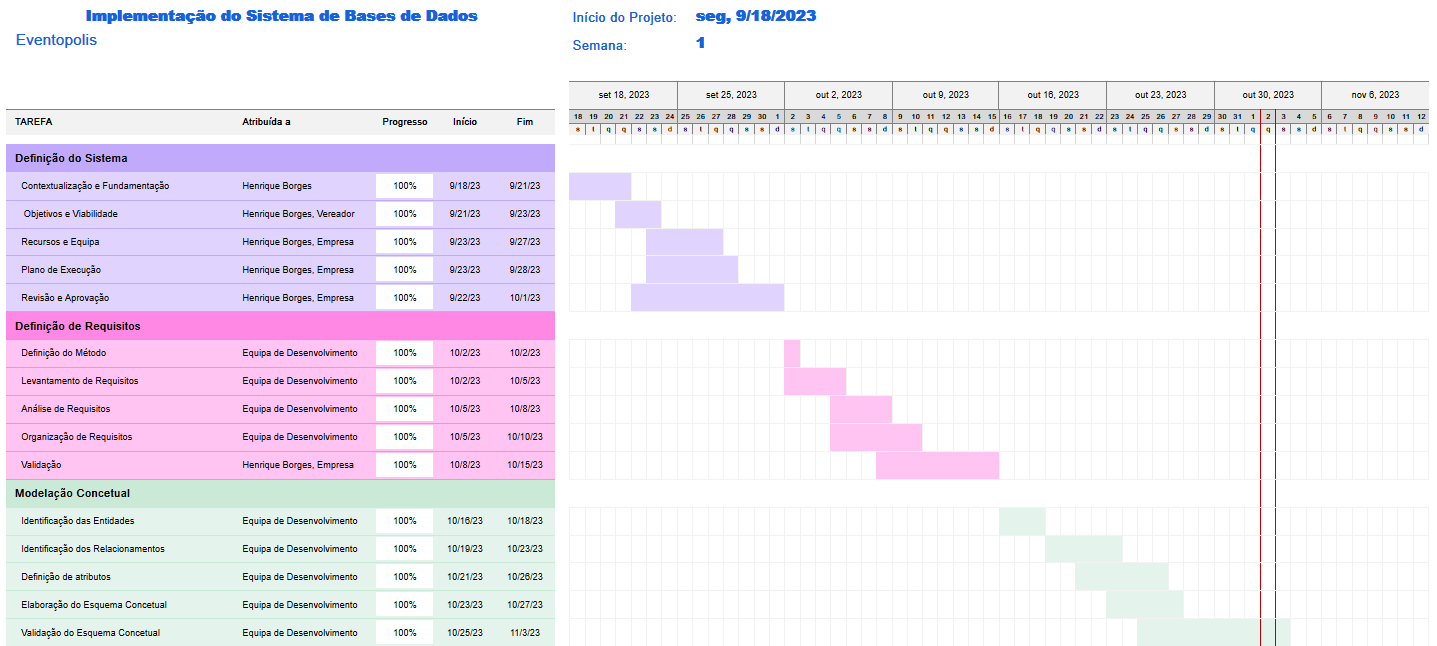
\includegraphics[width=6.2in]{images/GANTT_c1.png}
            \caption{Diagrama de GANTT com conteúdos da primeira fase do Trabalho}
        \end{figure}
    
    \section{Estrutura do Relatório}

    Após a introdução, seguir-se-ão mais dois capítulos, designadamente, metodologia e conclusão,
    acompanhados por um capítulo complementar para potenciais anexos.
    Na metodologia, abordaremos uma secção para cada fase do ``ciclo de vida'' do desenvolvimento de bases de dados,
    nomeadamente a definição de requisitos e modelação conceptual\footnote{De notar que este relat\'orio n\~ao abrange nas fases de modela\c{c}\~ao
        l\'ogica nem implementa\c{c}\~ao f\'isica, logo, n\~ao ser\~ao encontradas nesta fase do relat\'orio.}.
        
    A conclusão seguirá os padrões convencionais de tal secção, fornecendo um breve
    resumo dos resultados finais e indicando as próximas etapas necessárias para o sucesso do trabalho.
    Prosseguimos com o esclarecimento de siglas e abreviaturas e, finalmente, o capítulo de anexos,
    que pode conter \textit{scripts}, imagens de diagramas finais, entre outros.
        
%==========================================================================
% END INTRODUCTION
%==========================================================================
\chapter{Metodologia}
    \section{Defini\c{c}\~ao de Requisitos}
        \subsection{M\'etodo de Levantamento e de An\'alise de Requisitos Adotados}
        Com o objetivo de determinar os objetivos a serem alcançados pelo SBD,
        foram agendadas diversas reuniões com o Prof.\ Dr.\ Henrique Borges, onde foram discutidas
        várias questões pertinentes. No final destas reuniões, é previsto obter-se uma compreensão
        abrangente dos requisitos a serem implementados.
        \subsection{Organiza\c{c}\~ao dos Requisitos Levantados}
        \subsubsection{Requisitos de Descri\c{c}\~ao}
        \begin{table}[H]
    \centering
    \resizebox{\columnwidth}{!}{%
    \begin{tabular}{|l|l|l|>{\raggedright\arraybackslash}p{7cm}|l|l|l|}
    \hline
        Nr & ~ & Data e Hora & Descrição & Área & Fonte & Analista \\ \hline
        RD01 & 1 & 12:29 & Cada evento deve ter um identificador, uma descrição
        do mesmo, a data de início e de fim e pode ter, ou não, a capacidade &
        Eventos & Henrique Borges & Aurora Matrix \\ \hline
        RD02 & 2 & 12:30 & Cada funcionário deve ter um identificador, nome,
        NIF, data de nascimento, email, lista de telemoveis e morada (rua,
        localidade, código-postal & Eventos & Henrique Borges & Aurora Matrix
        \\ \hline RD03 & 3 & 12:31 & Cada venda deve ter um identificador, o
        valor total da venda, a quantidade de artigos na mesma e a data da
        venda & Eventos & Henrique Borges & Aurora Matrix \\ \hline
        RD04 & 4 & 12:32 & Cada participante dever ter um identificador, nome,
        NIF (opcional), data de nascimento, email (opcional), lista de números
        de telemóvel e opcionalmente, morada (rua, localidade, código-postal) &
        Eventos & Henrique Borges & Aurora Matrix \\ \hline RD05 & 5 & 12:33 &
        Cada artigo deve ter um identificador, nome, descrição do mesmo, preço
        e stock & Eventos & Henrique Borges & Aurora Matrix \\ \hline
        RD06 & 6 & 12:34 & Cada fornecedor deve ter um identificador, nome,
    IBAN, email, contacto (a pessoa que contactamos na empresa e o seu número
    de telemóvel), lista de números de telemóvel, morada (rua, localidade,
    código-postal) & Eventos & Henrique Borges & Aurora Matrix \\ \hline
    \end{tabular}%
    }
            \caption{Requisitos de Descrição}
\end{table}
        \newpage
        \subsubsection{Requisitos de Manipula\c{c}\~ao}
\begin{table}[H]
    \centering
    \resizebox{\columnwidth}{!}{%
    \begin{tabular}{|l|l|l|l|l|l|l|}
    \hline
        Nr & ~ & Data e Hora & Descrição & Área & Fonte & Analista \\ \hline
        RM01 & 10 & 12:37 & O administrador deve conseguir consultar qual funcionário gere qual & Eventos & Henrique Borges & Aurora Matrix \\ \hline
        RM02 & 11 & 12:38 & Um funcionário deve ser capaz de consultar qual é o funcionário que o gere & Eventos & Henrique Borges & Aurora Matrix \\ \hline
        RM03 & 12 & 12:39 & Um funcionário deve ser capaz de consultar que funcionário(s) gere & Eventos & Henrique Borges & Aurora Matrix \\ \hline
        RM04 & 13 & 12:40 & O administrador deve ser capaz de consultar as vendas efetuadas por um funcionário específico & Eventos & Henrique Borges & Aurora Matrix \\ \hline
        RM05 & 14 & 12:41 & O administrador deve ser capaz de consultar todas as vendas efetuadas & Eventos & Henrique Borges & Aurora Matrix \\ \hline
        RM06 & 15 & 12:42 & Um funcionário deve ser capaz de consultar as vendas que efetuou & Eventos & Henrique Borges & Aurora Matrix \\ \hline
        RM07 & 16 & 12:43 & O administrador deve ser capaz de consultar os artigos numa venda & Eventos & Henrique Borges & Aurora Matrix \\ \hline
        RM08 & 17 & 12:44 & O administrador deve ser capaz de consultar todos os artigos que estão numa venda & Eventos & Henrique Borges & Aurora Matrix \\ \hline
        RM09 & 18 & 12:45 & Um funcionário deve ser capaz de consultar os artigos numa venda & Eventos & Henrique Borges & Aurora Matrix \\ \hline
        RM10 & 19 & 12:46 & O administrador deve ser capaz de consultar todos os artigos & Eventos & Henrique Borges & Aurora Matrix \\ \hline
        RM11 & 20 & 12:47 & O administrador deve ser capaz de consultar os participantes de um evento & Eventos & Henrique Borges & Aurora Matrix \\ \hline
        RM12 & 21 & 12:48 & O administrador deve ser capaz de consultar todos os participantes em todos os eventos & Eventos & Henrique Borges & Aurora Matrix \\ \hline
        RM13 & 22 & 12:49 & O administrador deve ser capaz de consultar o participante de uma venda específica & Eventos & Henrique Borges & Aurora Matrix \\ \hline
        RM14 & 23 & 12:50 & Um funcionário deve ser capaz de consultar o participante de uma venda que efetuou & Eventos & Henrique Borges & Aurora Matrix \\ \hline
        RM15 & 24 & 12:51 & O administrador deve ser capaz de consultar todas as vendas de um participante & Eventos & Henrique Borges & Aurora Matrix \\ \hline
        RM16 & 25 & 12:52 & O administrador deve ser capaz de consultar o fornecedor de um certo artigo & Eventos & Henrique Borges & Aurora Matrix \\ \hline
        RM17 & 26 & 12:53 & O administrador deve ser capaz de consultar os passados fornecedores de um certo artigo & Eventos & Henrique Borges & Aurora Matrix \\ \hline
        RM18 & 27 & 12:54 & O administrador deve ser capaz de consultar todos os fornecedores & Eventos & Henrique Borges & Aurora Matrix \\ \hline
        RM19 & 28 & 12:55 & O administrador deve ser capaz de consultar todos os funcionários & Eventos & Henrique Borges & Aurora Matrix \\ \hline
        RM20 & 29 & 12:56 & O administrador deve ser capaz de consultar todos os eventos & Eventos & Henrique Borges & Aurora Matrix \\ \hline
        RM21 & 30 & 12:57 & O administrador deve ser capaz de consultar o valor de vendas num dia particular & Eventos & Henrique Borges & Aurora Matrix \\ \hline
        RM22 & 31 & 12:58 & Deve ser possível determinar qual é o participante com maior valor de vendas & Eventos & Henrique Borges & Aurora Matrix \\ \hline
        RM23 & 32 & 12:59 & Deve ser possível determinar qual é o evento com maior volume de vendas & Eventos & Henrique Borges & Aurora Matrix \\ \hline
        RM24 & 33 & 13:00 & Deve ser possível determinar qual foi o evento com maior participação & Eventos & Henrique Borges & Aurora Matrix \\ \hline
        RM25 & 34 & 13:01 & Os funcionários devem ser capazes de alterar as informações de um participante & Eventos & Henrique Borges & Aurora Matrix \\ \hline
        RM26 & 36 & 13:03 & No final do dia o sistema deve enviar um email ao Henrique Borges com o relatório de vendas & Eventos & Henrique Borges & Aurora Matrix \\ \hline
        RM27 & 37 & 13:04 & No final do dia o sistema deve enviar um email ao Henrique Borges com a afluência do evento & Eventos & Henrique Borges & Aurora Matrix \\ \hline
        RM28 & 38 & 13:05 & Um participante é inserido na base de dados quando compra um bilhete & Eventos & Henrique Borges & Aurora Matrix \\ \hline
        RM29 & 39 & 13:06 & Se o evento for gratuito a venda do bilhete deve ser registada na mesma mas com o valor a 0 & Eventos & Henrique Borges & Aurora Matrix \\ \hline
        RM30 & 40 & 13:07 & Não podem ser vendidos mais bilhetes para um evento do que a capacidade do mesmo & Eventos & Henrique Borges & Aurora Matrix \\ \hline
        RM31 & 42 & 13:09 & Os funcionários devem poder verificar o histórico de vendas de um participante & Eventos & Henrique Borges & Aurora Matrix \\ \hline
        RM32 & 44 & 13:12 & O administrador deve ser capaz de saber quais eventos decorreram num determinado período de tempo & Eventos & Henrique Borges & Aurora Matrix \\ \hline
        RM33 & 45 & 13:13 & O administrador deve ser capaz de consultar qual foi o funcionário que vendeu mais bilhetes num dado evento & Eventos & Henrique Borges & Aurora Matrix \\ \hline
    \end{tabular}%
}
    \caption{Requisitos de Manipulação}
\end{table}
        \newpage
        \subsubsection{Requisitos de Controlo}
        \begin{table}[H]
    \centering
    \resizebox{\columnwidth}{!}{%
    \begin{tabular}{|l|l|l|>{\raggedright\arraybackslash}p{8cm}|l|l|l|}
    \hline
        Nr & ~ & Data e Hora & Descrição & Área & Fonte & Analista \\ \hline
        RC01 & 7 & 12:35 & O administrador do sistema é o Henrique Borges & Eventos & Henrique Borges & Aurora Matrix \\ \hline
        RC02 & 8 & 12:36 & Herr Otto Mustermann e Maria Ivanovna Ivanova são também administradores & Eventos & Henrique Borges & Aurora Matrix \\ \hline
        RC03 & 9 & 12:36 & Herr Mustermann só tem acesso à base de dados entre as 15:30 e as 19:30 & Eventos & Henrique Borges & Aurora Matrix \\ \hline
        RC04 & 35 & 13:02 & Os funcionários não devem ter acesso ao valor de vendas de cada evento & Eventos & Henrique Borges & Aurora Matrix \\ \hline
        RC05 & 41 & 13:08 & O acesso à base de dados só está disponível das 07:00 às 02:00 & Eventos & Henrique Borges & Aurora Matrix \\ \hline
        RC06 & 43 & 13:10 & Os funcionários só podem aceder à base de dados se um evento estiver a decorrer & Eventos & Henrique Borges & Aurora Matrix \\ \hline
    \end{tabular}%
}
        \caption{Requisitos de Controlo}
        \end{table}
        \subsubsection{Análise e Validação Geral dos Requisitos}
        Depois do levantamento dos requisitos, marcou-se uma reunião no intuito de
        o pessoal externo tomar conhecimento dos requisitos documentados.

        Essa reunião, por sua vez, foi realizada com sucesso, e o pessoal interno
        mostrou-se satisfeito com o progresso e nível de detalhe a que os membros
        da equipa de desenvolvimento de BD chegaram, especialmente o Prof.\ Dr.\ Henrique
        Borges, que viu muito potencial neste projeto.
    \newpage
    \section{Modela\c{c}\~ao Conceptual}
        \subsection{Identificação Conceptual}
             Após analisar os requisitos anotados, a equipa de desenvolvimento procedeu com a 
             modelação conceptual do SBD, tendo iniciado pela identificação das entidades,
             relacionamentos e os atributos de cada uma.
             \subsubsection{Entidades}
             \begin{itemize}
                 \item{\textbf{Evento:}} 
                     \begin{itemize}
                         \item{ID} 
                         \item{Descrição}
                         \item{DataInicio}
                         \item{DataFim}
                         \item{Capacidade}
                     \end{itemize}
                 \item{\textbf{Funcionário:}}
                     \begin{itemize}
                         \item{ID}
                         \item{Nome}
                         \item{NIF}
                         \item{DataNascimento}
                         \item{Email}
                         \item{NTelemovel}
                         \item{Morada}
                     \end{itemize}
                 \item{\textbf{Venda:}}
                     \begin{itemize}
                         \item{ID}
                         \item{Valor}
                         \item{Quantidade}
                         \item{Data}
                     \end{itemize}
                 \item{\textbf{Participante:}}
                     \begin{itemize}
                         \item{ID}
                         \item{Nome}
                         \item{NIF}
                         \item{DataNascimento}
                         \item{Email}
                         \item{NTelemovel}
                         \item{Morada}
                     \end{itemize}
                 \item{\textbf{Artigo:}}
                     \begin{itemize}
                         \item{ID}
                         \item{Nome}
                         \item{Descrição}
                         \item{Preço}
                         \item{Stock}
                     \end{itemize}
                 \item{\textbf{Fornecedor:}}
                     \begin{itemize}
                         \item{ID}
                         \item{Nome}
                         \item{IBAN}
                         \item{Email}
                         \item{Contacto}
                         \item{NTelemovel}
                         \item{Morada}
                     \end{itemize}
             \end{itemize}
             \subsubsection{Relacionamentos}
             \begin{itemize}
                 \item{Evento emprega Funcionário:}
                 \item{Funcionário gere Funcionário:}
                 \item{Funcionário realiza Venda:}
                 \item{Venda contem Artigo:}
                     \begin{itemize}
                        \item{Valor}
                        \item{Quantidade}
                     \end{itemize}
                 \item{Venda para Participante:}
                 \item{Artigo fornecido por Fornecedor:}
                     \begin{itemize}
                        \item{Data}
                        \item{Quantidade}
                     \end{itemize}
                 \item{Artigo encomendado do Fornecedor:}
                     \begin{itemize}
                        \item{Data}
                        \item{Quantidade}
                     \end{itemize}
             \end{itemize}
        \subsection{Modelo Conceptual}
        Consoante os resultados da subsecção anterior, temos o seguinte diagrama ER,
        concebido na ferramenta BrModelo\footnote{No anexo \ref{chendiag} podemos ver
        o diagrama equivalente em notação de Peter Chen}:
        \begin{figure}[H]
            \centering
            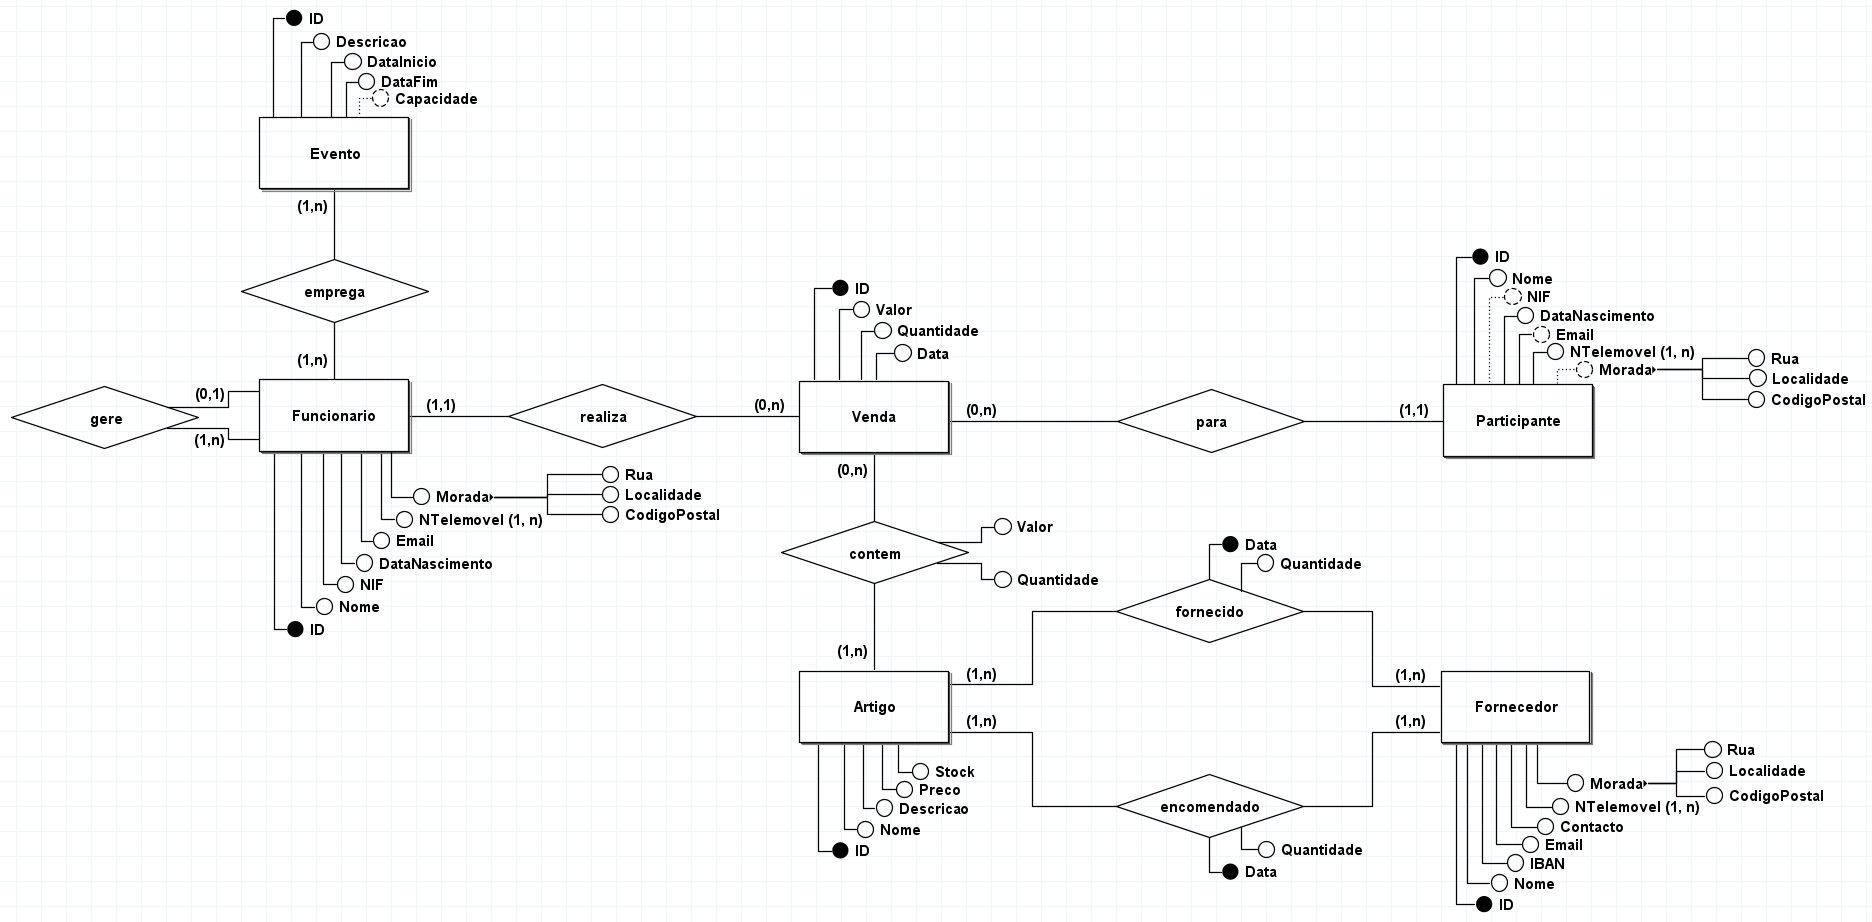
\includegraphics[width=4.75in]{images/Conceitual_Com_Atributos.png}
            \caption{Diagrama Conceitual}
        \end{figure}
        
        

    
%==========================================================================
% BEGIN CONCLUSÕES DE TRABALHO FUTURO
%==========================================================================

\chapter{Conclusões e Trabalho Futuro}
    

%==========================================================================
% END CONCLUSÕES DE TRABALHO FUTURO
%==========================================================================

%==========================================================================
% BEGIN REFERÊNCIAS
%==========================================================================

%% Changes biblibography name
%% Portuguese babel default : "Bibliografia"
%% Personally I prefer "Referências"
\renewcommand\bibname{Referências}

%% https://www.overleaf.com/learn/latex/bibliography_management_with_bibtex
\nocite{*}
\printbibliography


%==========================================================================
% END REFERÊNCIAS
%==========================================================================

%==========================================================================
% BEGIN LISTA DE SIGLAS E ACRÓNIMOS
%==========================================================================

%% Portuguese babel does not translate this environment
\renewcommand{\nomname}{Lista de Siglas e Acrónimos}

%% Text that can be shown before acronyms list
\renewcommand{\nompreamble}{}

%% acronyms
\nomenclature[01]{\textbf{BD}}{Base(s) de Dados}
\nomenclature[02]{\textbf{ER}}{Entity-Relationship}
\nomenclature[03]{\textbf{SBD}}{Sistema de Bases de Dados}
\nomenclature[04]{\textbf{SGBD}}{Sistema de Gestão de Bases de Dados}

%% Show acronyms
\printnomenclature



%==========================================================================
% END LISTA DE SIGLAS E ACRÓNIMOS
%==========================================================================


%==========================================================================
% BEGIN ANEXOS
%==========================================================================

%% Why \addchap, instead of \chapter? 
%%addchap has no numbering but appears in table of contents.
\chapter{Anexos}
    
    %% section version of \addchap
    \section{Anexo 1} \label{GANTT}
        \begin{figure}[h]
            \centering
            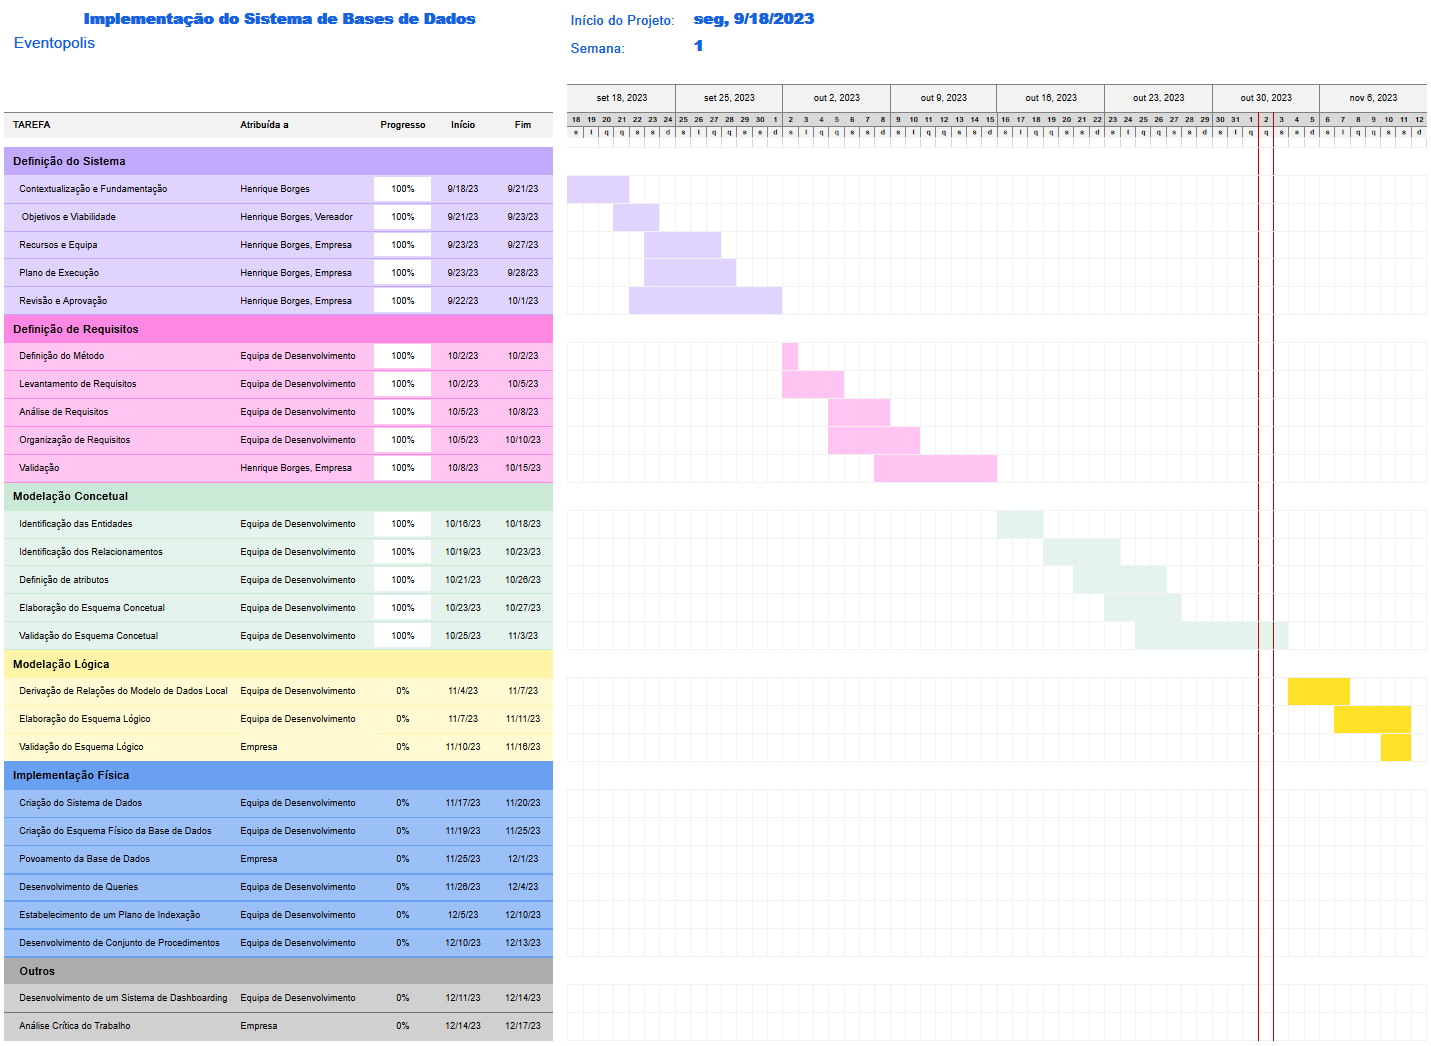
\includegraphics[width=6.2in]{images/GANTT.png}
        \end{figure}
\newpage
    \section{Anexo 2} \label{GANTT_c2}
        \begin{figure}[h]
            \centering
            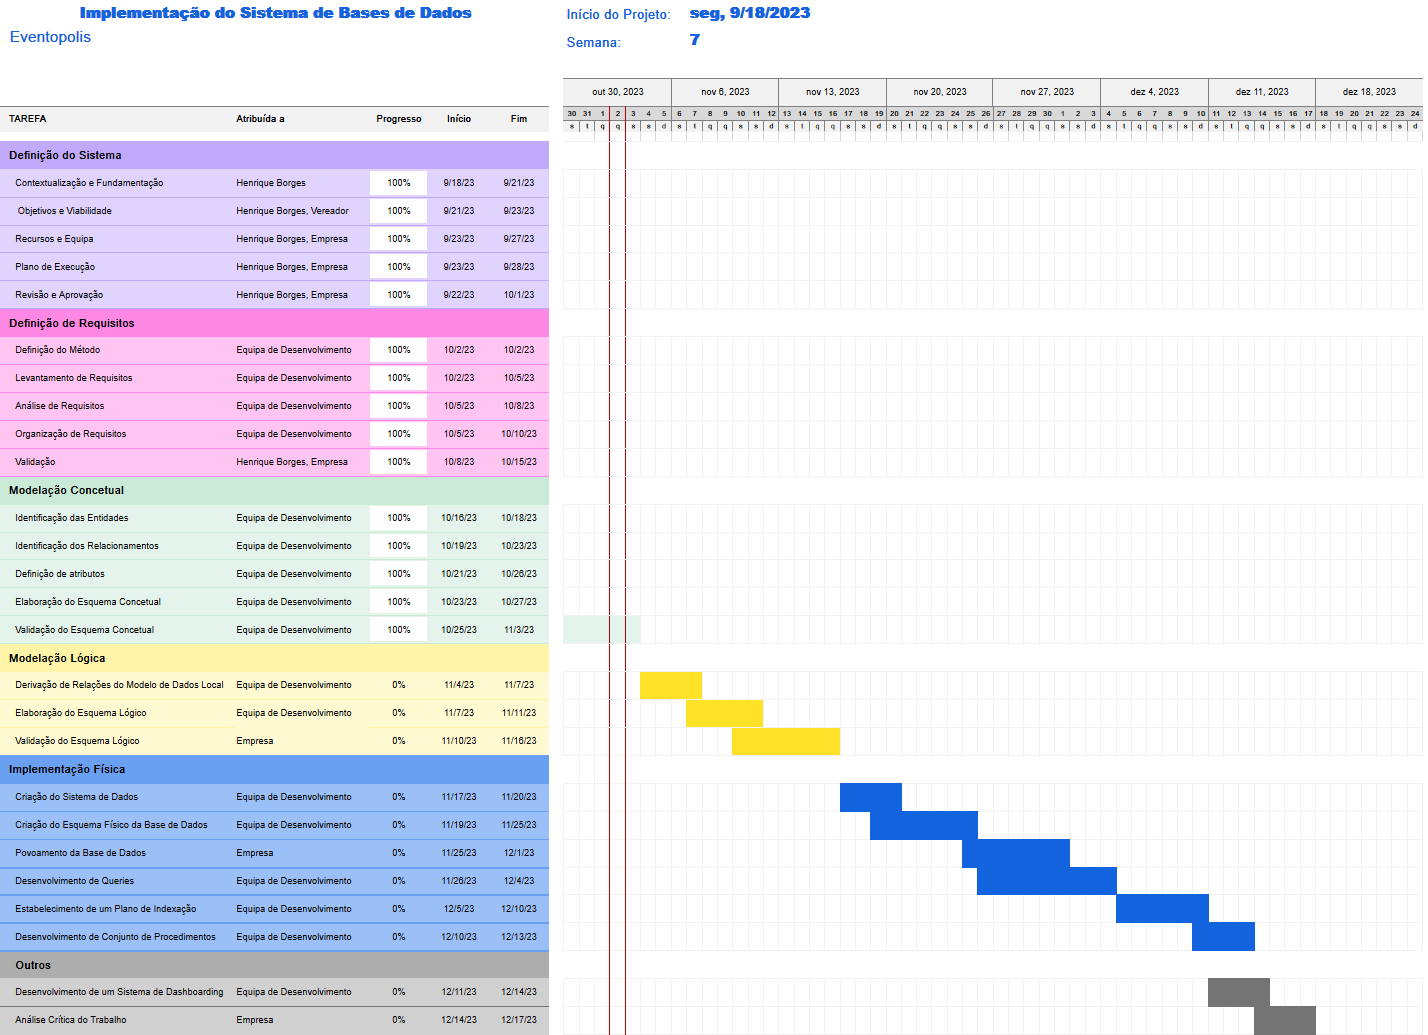
\includegraphics[width=6.2in]{images/GANTT_c2.png}
        \end{figure}
\newpage
    \section{Anexo 3} \label{chendiag}
    \usetikzlibrary{er,positioning}
\begin{tikzpicture}[auto,node distance=1.5cm]
  \node[entity] (node1) {event}
    [grow=up,sibling distance=3cm]
    child {node[attribute] {\underline{id}}}
    child {node[attribute] {description}}
    child {node[attribute] {capacity}}
    child {node[attribute] {start\_date}}
    child {node[attribute] {end\_date}};
  \node[relationship] (rel1) [below = of node1] {employs};
  \node[entity] (node2) [below = of rel1]	{employee};
  \node[relationship] (rel2) [below = of node2] {manages};
  \path (rel1) edge node {N} (node1)
    edge	 node {M}	(node2);
  \path (rel2) edge node {1} (node2)
    edge     node {  N}   (node2);
\end{tikzpicture}
\end{document}

%==========================================================================
% END ANEXOS
%==========================================================================
\end{document}
